\subsection{Tablas de enclavamientos}
	\label{sec:tablas}
	Históricamente, tanto los enclavamientos mecánicos como los electromecánicos se han definido mediante tablas de enclavamientos \cite{INTERLOCKING_BASIC,RITO,IRSE,Paper_204,Paper_205}, las cuales luego pueden ser usadas para definir la logística de la red. Es por eso que el personal técnico está muy capacitado tanto en la lectura de la tabla como en su elaboración.
	
	Cada ruta es definida junto con los elementos ferroviarios que la condicionan y los estados que deben tener los mismos para que la ruta sea habilitada. Además, se explicita cada una de las rutas que entrarían en conflicto con la ruta en cuestión. A modo de ejemplo se presenta en la Figura \ref{fig:funcional_1} como se realiza la asignación de rutas en un cambio de vías.
	
	\begin{figure}[h]
		\centering
		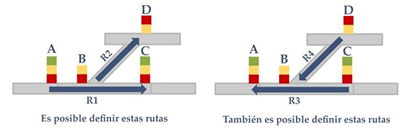
\includegraphics[width=1\textwidth]{Figuras/rutas.PNG}
		\centering\caption{Ejemplo de asignación de rutas.}
		\label{fig:funcional_1}
	\end{figure}
	
	Si el trazado de vías fuese utilizado para circular únicamente de izquierda a derecha, podemos definir únicamente dos rutas. La primera será la ruta R1, desde la señal A hasta la señal C. La segunda ruta R2 se define desde la señal B hasta la señal D, utilizando el cambio de vía a reverso. Ambas rutas quedan definidas en la Tabla \ref{Tab:funcional_2}.
	
	\begin{table}[!h]
		{
			\caption{Tabla de enclavamientos (rutas de izquierda a derecha).}
			\label{Tab:funcional_2}
			\centering
			%\small
			%\centering
			\begin{center}
				\resizebox{0.75\textwidth}{!}{
					\begin{tabular}{ c c c }
						\hline	
						Ruta & Señal de entrada & Señal de salida \\	
						\hline
						R$_1$ & Señal$_{\text{A}}$ & Señal$_{\text{C}}$ \\
						R$_2$ & Señal$_{\text{B}}$ & Señal$_{\text{D}}$ \\
						%\hline
					\end{tabular}
				}
			\end{center}
		}    
	\end{table}
	
	De forma análoga, podríamos analizar el mismo trazado de vías asumiendo que las formaciones circularán estrictamente de derecha a izquierda, definiendo otro nuevo conjunto de rutas. Sumando así las rutas R3 y R4 como se visualiza en la Tabla \ref{Tab:funcional_3}
	
	\begin{table}[!h]
		{
			\caption{Tabla de enclavamientos (rutas de derecha a izquierda).}
			\label{Tab:funcional_3}
			\centering
			%\small
			%\centering
			\begin{center}
				\resizebox{0.75\textwidth}{!}{
					\begin{tabular}{ c c c }
						\hline	
						Ruta & Señal de entrada & Señal de salida \\	
						\hline
						R$_3$ & Señal$_{\text{C}}$ & Señal$_{\text{A}}$ \\
						R$_4$ & Señal$_{\text{D}}$ & Señal$_{\text{B}}$ \\
						%\hline
					\end{tabular}
				}
			\end{center}
		}    
	\end{table}
	
	Ambas tablas de enclavamiento (Tabla \ref{Tab:funcional_2} y Tabla \ref{Tab:funcional_3}) son válidas, dependiendo del uso que se le quiera dar a la infraestructura. Incluso podemos notar que ambas tablas están incompletas porque una tabla no contempla los casos que contempla la otra y viceversa. Por lo tanto, es posible definir una nueva tabla de enclavamientos como la conjunción de ambas, como se muestra en la Tabla \ref{Tab:funcional_4}, especificando las rutas conflictivas.
	
	\begin{table}[!h]
		{
			\caption{Tabla de enclavamientos completa.}
			\label{Tab:funcional_4}
			\centering
			%\small
			%\centering
			\begin{center}
				\resizebox{1\textwidth}{!}{
					\begin{tabular}{ c c c c }
						\hline	
						Ruta & Señal de entrada & Señal de salida & Rutas conflictivas \\	
						\hline
						R$_1$ & Señal$_{\text{A}}$ & Señal$_{\text{C}}$ & R$_2$, R$_3$ y R$_4$\\
						R$_2$ & Señal$_{\text{B}}$ & Señal$_{\text{D}}$ & R$_1$, R$_3$ y R$_4$\\
						R$_3$ & Señal$_{\text{C}}$ & Señal$_{\text{A}}$ & R$_1$, R$_2$ y R$_4$\\
						R$_4$ & Señal$_{\text{D}}$ & Señal$_{\text{B}}$ & R$_1$, R$_2$ y R$_3$\\
						%\hline
					\end{tabular}
				}
			\end{center}
		}    
	\end{table}